%!TEX root = ../main.tex

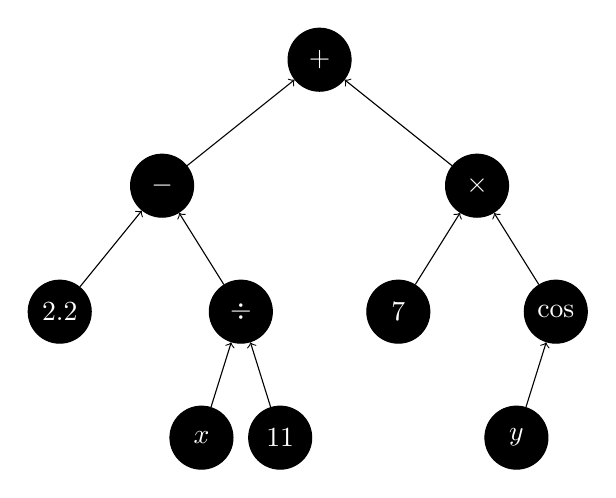
\begin{tikzpicture}[%
    node/.style = {circle, draw, minimum size = 0.8cm, align = flush center, inner sep = 0pt, fill = black, text = white},
    y = 0.8cm]

    \node[node] (x) at (5, 0) {$x$};
    \node[node] (11) at (6, 0) {$11$};
    \node[node] (y) at (9, 0) {$y$};
    \node[node] (div) at (5.5, 2) {$\div$};
    \node[node] (22) at (3.2, 2) {$2.2$};
    \node[node] (7) at (7.5, 2) {$7$};
    \node[node] (cos) at (9.5, 2) {$\cos$};
    \node[node] (sub) at (4.5, 4) {$-$};
    \node[node] (times) at (8.5, 4) {$\times$};
    \node[node] (plus) at (6.5, 6) {$+$};

    \draw[->] (x) -- (div);
    \draw[->] (11) -- (div);
    \draw[->] (y) -- (cos);
    \draw[->] (22) -- (sub);
    \draw[->] (div) -- (sub);
    \draw[->] (7) -- (times);
    \draw[->] (cos) -- (times);
    \draw[->] (sub) -- (plus);
    \draw[->] (times) -- (plus);
\end{tikzpicture}
